\documentclass[aspectratio=169,11pt,t]{beamer}

% ============================================================
% Theme and typography
% ============================================================

\usetheme{Madrid}
\usecolortheme{default}
\usefonttheme{professionalfonts}

\setbeamertemplate{navigation symbols}{}
\setbeamertemplate{headline}{}

\setbeamertemplate{footline}{%
  \leavevmode\hbox{%
  \begin{beamercolorbox}[wd=.82\paperwidth,ht=2.5ex,dp=1.0ex,leftskip=.8em]{author in head/foot}
    CSCI 2406 --- Computer Architecture \& Organization (ARM / RISC Reference)
  \end{beamercolorbox}%
  \begin{beamercolorbox}[wd=.18\paperwidth,ht=2.5ex,dp=1.0ex,rightskip=.8em]{date in head/foot}
    \hfill\insertframenumber/\inserttotalframenumber
  \end{beamercolorbox}}
}

\setbeamersize{
  text margin left=0.65cm,
  text margin right=0.65cm
}

\setbeamerfont{frametitle}{size=\Large, series=\bfseries}
\setbeamerfont{block title}{size=\normalsize, series=\bfseries}
\setbeamertemplate{blocks}[rounded][shadow=false]

% Block vertical padding adjustments
\addtobeamertemplate{block begin}{\vspace{0.1em}}{\vspace{0.1em}}
\addtobeamertemplate{block end}{}{\vspace{0.2em}}

% Base list item separation
\setbeamertemplate{itemize/enumerate body begin}{\setlength{\itemsep}{4pt}}
\setbeamertemplate{itemize/enumerate subbody begin}{\setlength{\itemsep}{2pt}}

% ============================================================
% Packages
% ============================================================

\usepackage[T1]{fontenc}
\usepackage{lmodern}
\usepackage{amsmath}
\usepackage{booktabs}
\usepackage{array}
\usepackage{colortbl}
\usepackage{tikz}

\usetikzlibrary{
  arrows.meta,
  positioning,
  shapes.geometric,
  calc,
  decorations.pathreplacing
}

% ============================================================
% Colors
% ============================================================

\definecolor{navy}{RGB}{24,43,68}
\definecolor{deepblue}{RGB}{45,88,130}
\definecolor{lightblue}{RGB}{235,242,250}
\definecolor{softgray}{RGB}{245,247,250}
\definecolor{darkgray}{RGB}{25,28,32}
\definecolor{gold}{RGB}{200,145,35}

\setbeamercolor{palette primary}{bg=navy,fg=white}
\setbeamercolor{palette secondary}{bg=deepblue,fg=white}
\setbeamercolor{frametitle}{bg=navy,fg=white}
\setbeamercolor{title}{fg=white}
\setbeamercolor{subtitle}{fg=white}
\setbeamercolor{author}{fg=white}
\setbeamercolor{date}{fg=white}
\setbeamercolor{titlelike}{fg=white}
\setbeamercolor{block title}{bg=deepblue,fg=white}
\setbeamercolor{block body}{bg=lightblue,fg=darkgray}
\setbeamercolor{normal text}{fg=darkgray,bg=white}

% ============================================================
% Formatting shortcuts
% ============================================================

\setlength{\parskip}{0pt}

\newcommand{\key}[1]{\textbf{#1}}
\newcommand{\bits}[1]{\texttt{#1}}
\newcommand{\hex}[1]{\texttt{0x#1}}
\newcommand{\code}[1]{\texttt{#1}}

% Section divider macro
\newcommand{\sectiondivider}[2]{%
\begin{frame}[plain]
\begin{tikzpicture}[remember picture,overlay]
\fill[navy] (current page.south west) rectangle (current page.north east);
\fill[gold] (current page.south west) rectangle ([yshift=.15cm]current page.south east);
\end{tikzpicture}
\vspace{1.5cm}
\begin{minipage}{0.85\textwidth}
{\color{gold}\large\bfseries #1\par}
\vspace{0.3cm}
{\color{white}\fontsize{22}{26}\selectfont\bfseries #2\par}
\end{minipage}
\end{frame}
}

% ============================================================
% Metadata
% ============================================================

\title[Topic 1]{
  Computer Architecture \& Organization Fundamentals
}

\subtitle{
  Architecture vs. Organization, ISA vs. Microarchitecture,\\
  the Stored-Program Concept, and Memory Models
}

\author{
  Computer Architecture \& Organization
}

\date{Week 1}

% ============================================================
% Presentation Body (35 Frames Total)
% ============================================================

\begin{document}

% --- Slide 1: Title Slide ---
\begin{frame}[plain]
\begin{tikzpicture}[remember picture,overlay]
\fill[navy] (current page.south west) rectangle (current page.north east);
\fill[gold] (current page.south west) rectangle ([yshift=.18cm]current page.south east);
\end{tikzpicture}
\vspace{1.0cm}
\begin{minipage}{0.9\textwidth}
{\color{gold}\large\bfseries CSCI 2406: Lecture 01\par}
\vspace{0.3cm}
{\color{white}\fontsize{20}{24}\selectfont\bfseries Computer Architecture \& Organization Fundamentals\par}
\vspace{0.3cm}
{\color{lightblue}\normalsize Abstraction Layers, ISA vs.\ Microarchitecture, Stored-Program Concept, and Memory Architectures\par}
\vspace{0.6cm}
{\color{softgray}\small Computer Architecture \& Organization \quad\textbar\quad Week 1\par}
\end{minipage}
\end{frame}

% --- Slide 2: Course Information & Logistics ---
\begin{frame}{Course Information \& Administration}
    \begin{columns}[T]
        \begin{column}{0.5\textwidth}
            \begin{block}{Instructor Contact}
                \begin{itemize}
                    \item \key{Email}: \code{jburns@ada.edu.az}
                    \item \key{Office}: B317
                    \item \key{Office Hours}: Thursdays 11:00--15:00\\(or by appointment)
                    \item \textit{Note}: Avoid Blackboard messages for urgent matters.
                \end{itemize}
            \end{block}
        \end{column}
        \begin{column}{0.48\textwidth}
            \begin{block}{Classroom Expectations}
                \begin{itemize}
                    \item \key{The Golden Rule}: Once class commences and the instructor speaks, no outside conversations are permitted.
                    \item \key{Authentic Work}: Emphasize the \textit{why} alongside the \textit{what} and \textit{how}. Do not pass off AI-generated output as your own.
                \end{itemize}
            \end{block}
        \end{column}
    \end{columns}
\end{frame}

% --- Slide 3: Laboratory Tools & Simulation Environment ---
\begin{frame}{Tools, Emulation, and Assessments}
    \begin{columns}[T]
        \begin{column}{0.48\textwidth}
            \begin{block}{Software \& Emulation Stack}
                \begin{itemize}
                    \item \key{C \& ARM Assembly}: Core languages utilized for architecture programming.
                    \item \key{CPUlator}: Web-based ARM simulator (\url{https://cpulator.01xz.net/?sys=arm}) to inspect step-by-step register updates.
                    \item \key{QEMU}: Full-system emulator for AArch64 virtual execution.
                \end{itemize}
            \end{block}
        \end{column}
        \begin{column}{0.48\textwidth}
            \begin{block}{Evaluation \& Assignments}
                \begin{itemize}
                    \item Exams drawn directly from lecture slides, class notes, and lab problem sets.
                    \item 2 Individual Take-Home Assignments.
                    \item Peer discussion is encouraged, but all submitted code and write-ups must be strictly authentic work.
                \end{itemize}
            \end{block}
        \end{column}
    \end{columns}
\end{frame}

% --- Slide 4: Lecture Roadmap ---
\begin{frame}{Week 1 Technical Roadmap}
    \begin{block}{Foundational Focus}
        Understanding the bridge connecting high-level algorithms to the physical silicon execution substrate.
    \end{block}
    \vspace{0.4em}
    \begin{itemize}
        \item \key{Topic 1}: The Full Stack of Abstraction Layers
        \item \key{Topic 2}: Computer Architecture versus Computer Organization
        \item \key{Topic 3}: Instruction Set Architecture (ISA) versus Microarchitecture
        \item \key{Topic 4}: The Stored-Program Concept \& Execution Cycle
        \item \key{Topic 5}: Memory Models: von Neumann, Harvard, and Modified Harvard
        \item \key{Topic 6}: Grand Synthesis \& Interactive Self-Test Review
    \end{itemize}
\end{frame}

% ============================================================
% SECTION 1
% ============================================================
\sectiondivider{Section 01}{The Full Stack of\\Abstraction Layers}

% --- Slide 6: The Full Abstraction Stack ---
\begin{frame}{The 9 Levels of Computer Abstraction}
    Computers manage immense complexity by enforcing clean hierarchical interfaces:
    \vspace{0.2em}
    \begin{center}
        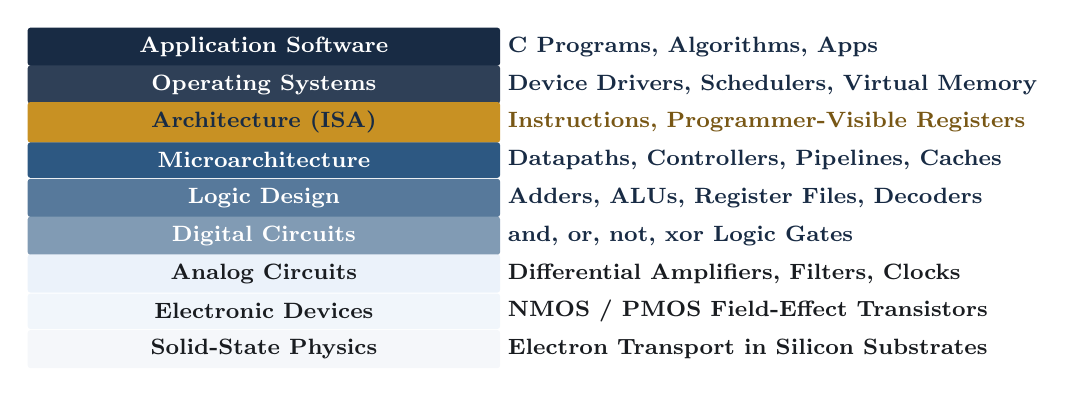
\begin{tikzpicture}[xscale=0.85, yscale=0.48, every node/.style={font=\footnotesize\bfseries}]
            % Layers
            \node[fill=navy, text=white, minimum width=6cm, minimum height=0.45cm, rounded corners=1pt] at (0,8) {Application Software};
            \node[fill=navy!90, text=white, minimum width=6cm, minimum height=0.45cm, rounded corners=1pt] at (0,7) {Operating Systems};
            \node[fill=gold, text=navy, minimum width=6cm, minimum height=0.45cm, rounded corners=1pt] at (0,6) {Architecture (ISA)};
            \node[fill=deepblue, text=white, minimum width=6cm, minimum height=0.45cm, rounded corners=1pt] at (0,5) {Microarchitecture};
            \node[fill=deepblue!80, text=white, minimum width=6cm, minimum height=0.45cm, rounded corners=1pt] at (0,4) {Logic Design};
            \node[fill=deepblue!60, text=white, minimum width=6cm, minimum height=0.45cm, rounded corners=1pt] at (0,3) {Digital Circuits};
            \node[fill=lightblue, text=darkgray, minimum width=6cm, minimum height=0.45cm, rounded corners=1pt] at (0,2) {Analog Circuits};
            \node[fill=lightblue!70, text=darkgray, minimum width=6cm, minimum height=0.45cm, rounded corners=1pt] at (0,1) {Electronic Devices};
            \node[fill=softgray, text=darkgray, minimum width=6cm, minimum height=0.45cm, rounded corners=1pt] at (0,0) {Solid-State Physics};

            % Right side descriptions
            \node[anchor=west, text=navy] at (3.5,8) {C Programs, Algorithms, Apps};
            \node[anchor=west, text=navy] at (3.5,7) {Device Drivers, Schedulers, Virtual Memory};
            \node[anchor=west, text=gold!60!black] at (3.5,6) {\textbf{Instructions, Programmer-Visible Registers}};
            \node[anchor=west, text=navy] at (3.5,5) {Datapaths, Controllers, Pipelines, Caches};
            \node[anchor=west, text=navy] at (3.5,4) {Adders, ALUs, Register Files, Decoders};
            \node[anchor=west, text=navy] at (3.5,3) {and, or, not, xor Logic Gates};
            \node[anchor=west, text=darkgray] at (3.5,2) {Differential Amplifiers, Filters, Clocks};
            \node[anchor=west, text=darkgray] at (3.5,1) {NMOS / PMOS Field-Effect Transistors};
            \node[anchor=west, text=darkgray] at (3.5,0) {Electron Transport in Silicon Substrates};
        \end{tikzpicture}
    \end{center}
\end{frame}

% --- Slide 7: The Central Divide ---
\begin{frame}{Where Software Meets Hardware}
    \begin{block}{The Strategic Core of CSCI 2406}
        Our course focuses on the critical boundary that translates logical intent into physical electrical actions: \key{Architecture} and \key{Microarchitecture}.
    \end{block}
    \vspace{0.4em}
    \begin{columns}[T]
        \begin{column}{0.48\textwidth}
            \begin{block}{Above the Boundary (Software)}
                \begin{itemize}
                    \item Applications compiled into machine binaries.
                    \item Operating systems managing hardware through architectural exception levels.
                    \item Completely portable across any hardware implementing the identical ISA.
                \end{itemize}
            \end{block}
        \end{column}
        \begin{column}{0.48\textwidth}
            \begin{block}{Below the Boundary (Hardware)}
                \begin{itemize}
                    \item Microarchitecture (datapaths and state controllers).
                    \item Digital circuits and gate-level logic.
                    \item Silicon fabrication nodes and thermal design power (TDP) constraints.
                \end{itemize}
            \end{block}
        \end{column}
    \end{columns}
\end{frame}

% ============================================================
% SECTION 2
% ============================================================
\sectiondivider{Section 02}{Computer Architecture vs.\\Computer Organization}

% --- Slide 9: Architecture Defined ---
\begin{frame}{What is Computer Architecture?}
    \key{Computer Architecture} defines the \key{externally visible capabilities and behavior} of the machine---the \key{\textit{what}}.
    \vspace{0.2em}
    \begin{itemize}
        \item The programmer-visible specification of the computer system.
        \item Establishes what the software is allowed to execute and what state changes occur.
        \item Determines the binary interface targeted by compilers and assembly programmers.
    \end{itemize}
    \vspace{0.3em}
    \begin{block}{Architectural Specifications Include:}
        \begin{itemize}
            \item The complete \key{Instruction Set Architecture (ISA)} vocabulary.
            \item Programmer-visible registers (\code{r0}--\code{r31}, program counter \code{pc}, status flags).
            \item Instruction encodings, data formats (byte, halfword, word), and addressing modes.
        \end{itemize}
    \end{block}
\end{frame}

% --- Slide 10: Organization Defined ---
\begin{frame}{What is Computer Organization?}
    \key{Computer Organization} describes the \key{internal hardware implementation} of the architecture---the \key{\textit{how}}.
    \vspace{0.2em}
    \begin{itemize}
        \item The physical arrangement of operational units and their logical interconnections.
        \item Defines how the machine physically performs the architectural operation.
        \item Completely transparent (invisible) to the programmer and machine software.
    \end{itemize}
    \vspace{0.3em}
    \begin{block}{Organizational Structures Include:}
        \begin{itemize}
            \item Datapaths, control units, ALUs, and multiplexer routing.
            \item Pipeline staging, branch prediction logic, and cache hierarchies (L1/L2/L3).
            \item Internal bus interfaces, clocking frequencies, and memory controller arbitration.
        \end{itemize}
    \end{block}
\end{frame}

% --- Slide 11: Direct Comparison Table ---
\begin{frame}{Architecture vs. Organization: Direct Contrast}
    \begin{table}[]
        \centering
        \small
        \begin{tabular}{p{5.5cm} p{6.5cm}}
            \toprule
            \textbf{Computer Architecture (\textit{What})} & \textbf{Computer Organization (\textit{How})} \\
            \midrule
            Programmer / Compiler view & Hardware engineer / Silicon designer view \\
            Functional contract and behavior & Physical implementation and datapath \\
            Changes slowly across generations & Evolves rapidly with silicon manufacturing nodes \\
            Example: Does an \code{mul} instruction exist? & Example: Is multiplication done via shift-and-add logic or a dedicated hardware multiplier? \\
            Specifies visible registers \& flags & Specifies pipeline stages, ALU internal circuits \\
            Software target (C, ARM assembly) & Hardware target (Verilog, VHDL, RTL) \\
            \bottomrule
        \end{tabular}
    \end{table}
\end{frame}

% --- Slide 12: Architectural Longevity Example ---
\begin{frame}{Real-World Continuity: The ARM Ecosystem}
    \begin{block}{The Economic Benefit of a Stable Architecture}
        Preserving the architecture allows software investments to persist indefinitely while the internal organization is completely overhauled for performance.
    \end{block}
    \vspace{0.3em}
    \begin{columns}[T]
        \begin{column}{0.48\textwidth}
            \begin{block}{Architectural Invariance}
                \begin{itemize}
                    \item The \key{AArch64 ISA} defines instructions like \code{add}, \code{ldr}, and \code{cbz}.
                    \item An ARM64 binary compiled in 2012 executes seamlessly on modern Apple M-series or AWS Graviton CPUs.
                \end{itemize}
            \end{block}
        \end{column}
        \begin{column}{0.48\textwidth}
            \begin{block}{Organizational Evolution}
                \begin{itemize}
                    \item 2012: In-order 2-wide pipelines, small 32\,KB L1 caches, 28\,nm process.
                    \item Modern: Out-of-order 8-wide superscalar engines, unified L3 caches, 3\,nm process.
                \end{itemize}
            \end{block}
        \end{column}
    \end{columns}
\end{frame}

% ============================================================
% SECTION 3
% ============================================================
\sectiondivider{Section 03}{ISA versus Microarchitecture}

% --- Slide 14: ISA as the Interface Language ---
\begin{frame}{The Instruction Set Architecture (ISA)}
    The \key{ISA} is the complete vocabulary of machine instructions supported by the hardware.
    \begin{itemize}
        \item All software running on a given processor must be expressed using its specific ISA.
        \item Different programs use different subsets, but all conform to the common ISA dictionary.
    \end{itemize}
    \vspace{0.3em}
    \begin{block}{The Architectural Contract: \code{add r1, r2, r3}}
        The ISA guarantees a single semantic state change:
        $$\text{Register } r_1 \leftarrow \text{Register } r_2 + \text{Register } r_3$$
        \begin{itemize}
            \item The architecture defines \textit{what} state update occurs upon completion.
            \item It does not state \textit{how} data moves across physical buses or wires inside the CPU.
        \end{itemize}
    \end{block}
\end{frame}

% --- Slide 15: Microarchitecture Execution Steps (No TikZ) ---
\begin{frame}{Microarchitecture: Executing \code{add r1, r2, r3}}
    \begin{block}{Register Transfer Steps for \code{add r1, r2, r3}}
        \begin{enumerate}
            \item \code{ra1 <- r2; ra2 <- r3} \hfill \textit{(Assert register read addresses)}
            \item \code{rd1 <- RegisterFile[ra1]; rd2 <- RegisterFile[ra2]} \hfill \textit{(Read operand values)}
            \item \code{alu\_control <- add} \hfill \textit{(Configure ALU operation multiplexers)}
            \item \code{alu\_result <- rd1 + rd2} \hfill \textit{(Execute 32-bit addition)}
            \item \code{reg\_write <- 1} \hfill \textit{(Assert register file write enable)}
            \item \code{RegisterFile[r1] <- alu\_result} \hfill \textit{(Commit result to destination register)}
        \end{enumerate}
    \end{block}
    \vspace{0.3em}
    \begin{itemize}
        \item \key{ISA View}: Add values in \code{r2} and \code{r3}; store sum into \code{r1}.
        \item \key{Microarchitecture View}: Sequence control signals, bus transfers, and ALU operations.
    \end{itemize}
\end{frame}

% --- Slide 16: Datapath Microarchitecture Diagram ---
\begin{frame}{Visualizing the Microarchitectural Datapath}
    \begin{center}
        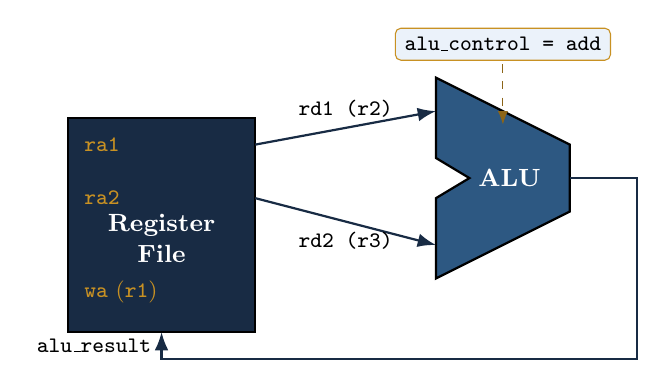
\begin{tikzpicture}[scale=0.85, every node/.style={font=\footnotesize}]
            % Register File
            \draw[thick, fill=navy, text=white] (0,0) rectangle (2.8,3.2);
            \node[text=white, font=\small\bfseries, align=center] at (1.4,1.4) {Register\\File};
            \node[text=gold, anchor=west] at (0.1,2.8) {\code{ra1}};
            \node[text=gold, anchor=west] at (0.1,2.0) {\code{ra2}};
            \node[text=gold, anchor=west] at (0.1,0.6) {\code{wa} (\code{r1})};
            
            % ALU
            \draw[thick, fill=deepblue, text=white] (5.5,0.8) -- (7.5,1.8) -- (7.5,2.8) -- (5.5,3.8) -- (5.5,2.6) -- (6.0,2.3) -- (5.5,2.0) -- cycle;
            \node[text=white, font=\small\bfseries] at (6.6,2.3) {ALU};
            
            % Routing Lines
            \draw[thick, -Latex, draw=navy] (2.8,2.8) -- node[above]{\code{rd1 (r2)}} (5.5,3.3);
            \draw[thick, -Latex, draw=navy] (2.8,2.0) -- node[below]{\code{rd2 (r3)}} (5.5,1.3);
            \draw[thick, -Latex, draw=navy] (7.5,2.3) -- (8.5,2.3) -- (8.5,-0.4) -- (1.4,-0.4) -- node[left]{\code{alu\_result}} (1.4,0);
            
            % Control signals
            \node[draw=gold, fill=lightblue, rounded corners=2pt] at (6.5,4.3) {\code{alu\_control = add}};
            \draw[dashed, -Latex, draw=gold!70!black] (6.5,4.0) -- (6.5,3.1);
        \end{tikzpicture}
    \end{center}
    \begin{itemize}
        \item Microarchitectures differ by doing this sequentially in multiple cycles or parallelized within single/pipelined cycles.
    \end{itemize}
\end{frame}

% --- Slide 17: One ISA, Many Microarchitectures ---
\begin{frame}{One ISA --- Multiple Hardware Realizations}
    \begin{table}[]
        \centering
        \small
        \begin{tabular}{p{3.2cm} p{4.0cm} p{4.2cm}}
            \toprule
            \textbf{Microarchitecture} & \textbf{Datapath Style} & \textbf{Design Objective} \\
            \midrule
            \key{Single-Cycle} & Every instruction takes 1 long clock cycle & Simple control; slow clock rate \\
            \key{Multi-Cycle} & Instructions take variable number of short cycles & Low hardware cost; reuse functional units \\
            \key{Pipelined (Classic 5-Stage)} & Overlap fetch, decode, execute, memory, writeback & Higher instruction throughput (1 inst/cycle ideal) \\
            \key{Superscalar Out-of-Order} & Multiple pipelines, dynamic instruction scheduling & Maximum performance for desktops/servers \\
            \bottomrule
        \end{tabular}
    \end{table}
    \vspace{0.2em}
    \begin{block}{Key Principle}
        All four microarchitectures execute the identical compiled ARM binary accurately.
    \end{block}
\end{frame}

% ============================================================
% SECTION 4
% ============================================================
\sectiondivider{Section 04}{The Stored-Program Concept}

% --- Slide 19: The Stored-Program Principle ---
\begin{frame}{The Stored-Program Concept}
    \begin{block}{Foundational Definition}
        Program instructions are encoded as binary numbers and stored in the exact same addressable memory subsystem alongside standard runtime data.
    \end{block}
    \vspace{0.4em}
    \key{Capabilities of a General-Purpose Computer}:
    \begin{itemize}
        \item \key{Store Information}: Holds data values and program sequences electronically.
        \item \key{Manipulate Information}: Performs mathematical and logical transformations via the ALU.
        \item \key{Make Decisions}: Alters control flow dynamically based on evaluated conditions (e.g., conditional branches).
    \end{itemize}
    \vspace{0.2em}
    \begin{alertblock}{Core Breakthrough}
        Reprogramming does not require physical rewiring; it simply requires loading new numbers into memory.
    \end{alertblock}
\end{frame}

% --- Slide 20: CPU and Memory Interface ---
\begin{frame}{The CPU--Memory Interface: Three Fundamental Buses}
    \begin{center}
        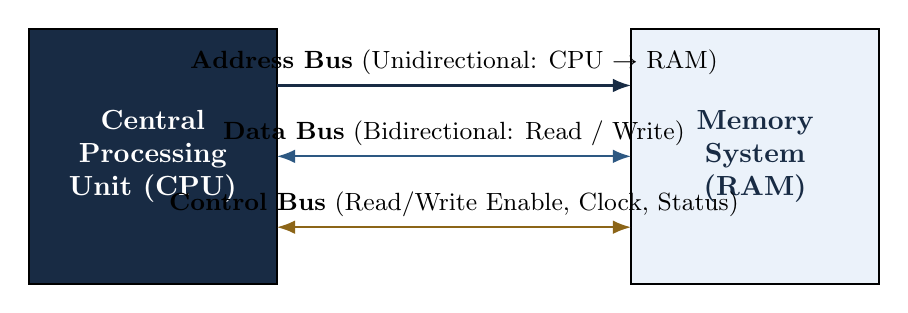
\begin{tikzpicture}[scale=0.9, every node/.style={font=\small}]
            % CPU Box
            \draw[thick, fill=navy, text=white] (0,0) rectangle (3.5,3.6);
            \node[text=white, font=\normalsize\bfseries, align=center] at (1.75,1.8) {Central\\Processing\\Unit (CPU)};
            
            % Memory Box
            \draw[thick, fill=lightblue, text=darkgray] (8.5,0) rectangle (12,3.6);
            \node[text=navy, font=\normalsize\bfseries, align=center] at (10.25,1.8) {Memory\\System\\(RAM)};
            
            % Buses
            \draw[thick, -Latex, draw=navy] (3.5,2.8) -- node[above]{\textbf{Address Bus} (Unidirectional: CPU $\rightarrow$ RAM)} (8.5,2.8);
            \draw[thick, Latex-Latex, draw=deepblue] (3.5,1.8) -- node[above]{\textbf{Data Bus} (Bidirectional: Read / Write)} (8.5,1.8);
            \draw[thick, Latex-Latex, draw=gold!70!black] (3.5,0.8) -- node[above]{\textbf{Control Bus} (Read/Write Enable, Clock, Status)} (8.5,0.8);
        \end{tikzpicture}
    \end{center}
    \begin{itemize}
        \item \key{Address Bus}: Selects the specific memory cell location to access.
        \item \key{Data Bus}: Transfers the numerical word to or from the selected cell.
        \item \key{Control Bus}: Dictates the direction of transfer (read vs. write) and timing signals.
    \end{itemize}
\end{frame}

% --- Slide 21: Memory Cell Indexing ---
\begin{frame}{Memory as an Array of Numbered Cells}
    \begin{columns}[T]
        \begin{column}{0.55\textwidth}
            \key{How Memory is Structured}:
            \begin{itemize}
                \item Memory is viewed logically as a contiguous 1-D array of cells.
                \item Each cell has a unique numerical \key{Address} and stores a \key{Value}.
                \item Address 4 holds value \code{3}.
                \item An address is simply an index; the data is the payload.
            \end{itemize}
        \end{column}
        \begin{column}{0.42\textwidth}
            \begin{center}
                \small
                \begin{tabular}{c|c|}
                    \toprule
                    \textbf{Address} & \textbf{Stored Value} \\
                    \midrule
                    0 & 7 \\
                    1 & 3 \\
                    2 & 15 \\
                    3 & 20 \\
                    \rowcolor{gold!20} 4 & \textbf{3} $\leftarrow$ Cell content \\
                    5 & 7 \\
                    6 & 3 \\
                    \bottomrule
                \end{tabular}
            \end{center}
        \end{column}
    \end{columns}
\end{frame}

% --- Slide 22: Dual Nature of Bits ---
\begin{frame}{Context Determines Meaning}
    \begin{block}{Bit Invariance Principle}
        A pattern of bits residing in a memory cell possesses no intrinsic, permanent identity. Its meaning is determined entirely by \key{how the CPU accesses and interprets it}.
    \end{block}
    \vspace{0.4em}
    Consider a 32-bit word stored in memory at location \hex{0x00001000}:
    \vspace{0.2em}
    \begin{itemize}
        \item If the \key{program counter (\code{pc})} points here $\rightarrow$ the CPU fetches and decodes it as an \key{ARM instruction}.
        \item If an \key{arithmetic load instruction} reads this address $\rightarrow$ the CPU treats it as a \key{signed / unsigned integer}.
        \item If a \key{pointer variable} holds this address $\rightarrow$ it is treated as a \key{memory reference}.
        \item If passed to a \key{display routine} $\rightarrow$ it is rendered as \key{ASCII/UTF-8 text characters}.
    \end{itemize}
\end{frame}

% --- Slide 23: The Machine Instruction Cycle ---
\begin{frame}{The Classical Machine Instruction Lifecycle}
    The processor continuously steps through code using the \key{program counter (\code{pc})}:
    \vspace{0.3em}
    \begin{center}
        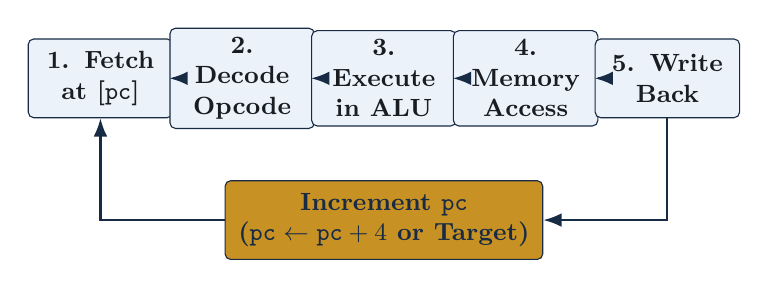
\begin{tikzpicture}[node distance=1.8cm, auto,
            stage/.style={rectangle, draw=navy, fill=lightblue, text=darkgray, font=\small\bfseries, text width=1.6cm, align=center, rounded corners=2pt, minimum height=1.0cm},
            arr/.style={draw=navy, -Latex, thick}]
            \node [stage] (fetch) {1. Fetch\\at [\code{pc}]};
            \node [stage, right of=fetch] (decode) {2. Decode\\Opcode};
            \node [stage, right of=decode] (exec) {3. Execute\\in ALU};
            \node [stage, right of=exec] (mem) {4. Memory\\Access};
            \node [stage, right of=mem] (wb) {5. Write\\Back};
            \node [stage, below of=exec, fill=gold, text=navy, text width=3.8cm] (pc) {Increment \code{pc}\\($\code{pc} \leftarrow \code{pc} + 4$ or Target)};
            
            \path [arr] (fetch) -- (decode);
            \path [arr] (decode) -- (exec);
            \path [arr] (exec) -- (mem);
            \path [arr] (mem) -- (wb);
            \path [arr] (wb) |- (pc);
            \path [arr] (pc) -| (fetch);
        \end{tikzpicture}
    \end{center}
    \vspace{0.1em}
    \begin{itemize}
        \item Because code is in memory, programs can be loaded, copied, relocated, or modified dynamically.
    \end{itemize}
\end{frame}

% ============================================================
% SECTION 5
% ============================================================
\sectiondivider{Section 05}{von Neumann vs. Harvard\\Architectures}

% --- Slide 25: von Neumann Architecture ---
\begin{frame}{The von Neumann Architecture}
    \begin{columns}[T]
        \begin{column}{0.55\textwidth}
            \key{Core Characteristics}:
            \begin{itemize}
                \item \key{Unified Memory}: A single address space containing both instructions and data.
                \item \key{Shared Bus System}: A single set of address, data, and control lines is shared.
                \item \key{Operation}: The CPU fetches an instruction, then subsequently accesses data using the same bus.
                \item Directly realizes the stored-program concept in its purest form.
            \end{itemize}
        \end{column}
        \begin{column}{0.42\textwidth}
            \begin{center}
                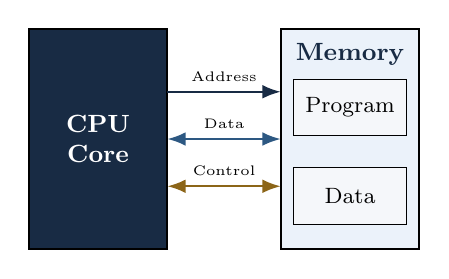
\begin{tikzpicture}[scale=0.8, every node/.style={font=\footnotesize}]
                    \draw[thick, fill=navy, text=white] (0,0) rectangle (2.2,3.5);
                    \node[text=white, font=\small\bfseries, align=center] at (1.1,1.75) {CPU\\Core};
                    
                    \draw[thick, fill=lightblue, text=darkgray] (4.0,0) rectangle (6.2,3.5);
                    \node[text=navy, font=\small\bfseries] at (5.1,3.1) {Memory};
                    \draw[fill=softgray] (4.2,1.8) rectangle (6.0,2.7);
                    \node at (5.1,2.25) {Program};
                    \draw[fill=softgray] (4.2,0.4) rectangle (6.0,1.3);
                    \node at (5.1,0.85) {Data};
                    
                    \draw[thick, -Latex, draw=navy] (2.2,2.5) -- node[above]{\tiny Address} (4.0,2.5);
                    \draw[thick, Latex-Latex, draw=deepblue] (2.2,1.75) -- node[above]{\tiny Data} (4.0,1.75);
                    \draw[thick, Latex-Latex, draw=gold!70!black] (2.2,1.0) -- node[above]{\tiny Control} (4.0,1.0);
                \end{tikzpicture}
            \end{center}
        \end{column}
    \end{columns}
\end{frame}

% --- Slide 26: Harvard Architecture ---
\begin{frame}{The Harvard Architecture}
    \begin{columns}[T]
        \begin{column}{0.55\textwidth}
            \key{Core Characteristics}:
            \begin{itemize}
                \item \key{Separated Memories}: Physically independent instruction and data memory modules.
                \item \key{Independent Buses}: Dedicated address, data, and control lines for each memory bank.
                \item \key{Parallel Operation}: CPU can fetch an instruction and read/write data operands \key{simultaneously}.
                \item Instruction and data words can have differing bit-widths and storage technologies.
            \end{itemize}
        \end{column}
        \begin{column}{0.42\textwidth}
            \begin{center}
                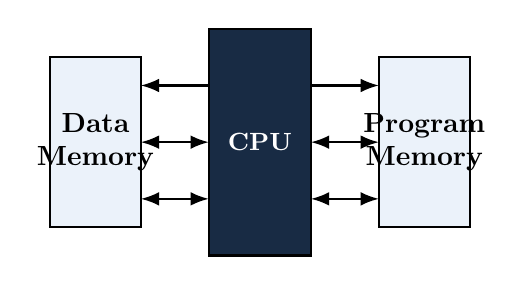
\begin{tikzpicture}[scale=0.72, every node/.style={font=\tiny}]
                    \draw[thick, fill=navy, text=white] (2.0,0) rectangle (3.8,4.0);
                    \node[text=white, font=\small\bfseries, align=center] at (2.9,2.0) {CPU};
                    
                    % Data Mem Left
                    \draw[thick, fill=lightblue] (-0.8,0.5) rectangle (0.8,3.5);
                    \node[font=\bfseries, align=center] at (0,2.0) {Data\\Memory};
                    
                    % Program Mem Right
                    \draw[thick, fill=lightblue] (5.0,0.5) rectangle (6.6,3.5);
                    \node[font=\bfseries, align=center] at (5.8,2.0) {Program\\Memory};
                    
                    % Data Bus Left
                    \draw[thick, -Latex] (2.0,3.0) -- (0.8,3.0);
                    \draw[thick, Latex-Latex] (2.0,2.0) -- (0.8,2.0);
                    \draw[thick, Latex-Latex] (2.0,1.0) -- (0.8,1.0);
                    
                    % Inst Bus Right
                    \draw[thick, -Latex] (3.8,3.0) -- (5.0,3.0);
                    \draw[thick, Latex-Latex] (3.8,2.0) -- (5.0,2.0);
                    \draw[thick, Latex-Latex] (3.8,1.0) -- (5.0,1.0);
                \end{tikzpicture}
            \end{center}
        \end{column}
    \end{columns}
\end{frame}

% --- Slide 27: Structural Separation vs Storage Location ---
\begin{frame}{Structural Separation: The Key Distinction}
    \begin{block}{The Fundamental Question}
        The decisive architectural issue is not simply where bytes are stored. It is \key{whether instruction access and data access are structurally separated}.
    \end{block}
    \vspace{0.4em}
    \begin{columns}[T]
        \begin{column}{0.48\textwidth}
            \begin{block}{Single Shared Bus (vN)}
                \begin{itemize}
                    \item Sequential access creates bus contention (\key{von Neumann bottleneck}).
                    \item Lower hardware routing cost and flexible memory budgeting.
                \end{itemize}
            \end{block}
        \end{column}
        \begin{column}{0.48\textwidth}
            \begin{block}{Dedicated Dual Buses (Harvard)}
                \begin{itemize}
                    \item Concurrent instruction fetch and operand read/write eliminates structural stalls.
                    \item Higher pin counts and rigid memory partition limits.
                \end{itemize}
            \end{block}
        \end{column}
    \end{columns}
\end{frame}

% --- Slide 28: Modified Harvard Architecture ---
\begin{frame}{The Modern Standard: Modified Harvard Architecture}
    Modern RISC systems (e.g., Apple M-series, ARM Cortex-A) merge both concepts:
    \vspace{0.2em}
    \begin{center}
        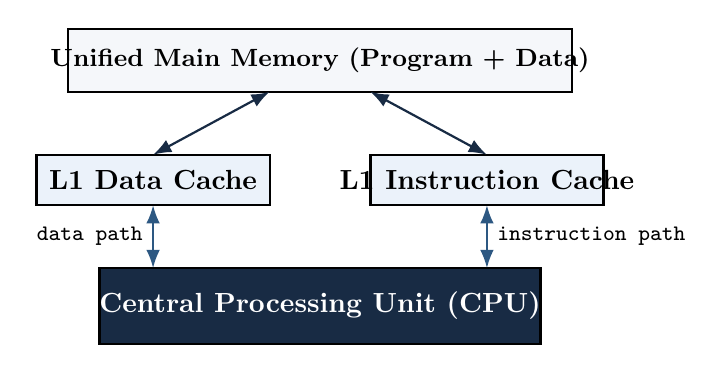
\begin{tikzpicture}[scale=0.8, every node/.style={font=\footnotesize}]
            % Main memory
            \draw[thick, fill=softgray, text=navy] (1,4.0) rectangle (9,5.0);
            \node[font=\small\bfseries, align=center] at (5,4.5) {Unified Main Memory (Program + Data)};
            
            % Split caches
            \draw[thick, fill=lightblue, text=darkgray] (0.5,2.2) rectangle (4.2,3.0);
            \node[font=\bfseries, align=center] at (2.35,2.6) {L1 Data Cache};
            \draw[thick, fill=lightblue, text=darkgray] (5.8,2.2) rectangle (9.5,3.0);
            \node[font=\bfseries, align=center] at (7.65,2.6) {L1 Instruction Cache};
            
            % CPU Box
            \draw[thick, fill=navy, text=white] (1.5,0.0) rectangle (8.5,1.2);
            \node[font=\normalsize\bfseries, text=white, align=center] at (5,0.6) {Central Processing Unit (CPU)};
            
            % Connectors
            \draw[thick, Latex-Latex, draw=deepblue] (2.35,1.2) -- node[left]{\code{data path}} (2.35,2.2);
            \draw[thick, Latex-Latex, draw=deepblue] (7.65,1.2) -- node[right]{\code{instruction path}} (7.65,2.2);
            \draw[thick, Latex-Latex, draw=navy] (2.35,3.0) -- (4.2,4.0);
            \draw[thick, Latex-Latex, draw=navy] (7.65,3.0) -- (5.8,4.0);
        \end{tikzpicture}
    \end{center}
    \vspace{-0.2em}
    \begin{itemize}
        \item \key{Internally}: Separate L1 caches yield Harvard pipeline throughput.
        \item \key{Externally}: Unified RAM preserves von Neumann software simplicity.
    \end{itemize}
\end{frame}

% --- Slide 29: Architecture Comparison Table ---
\begin{frame}{Comparison Summary: Memory Topologies}
    \begin{table}[]
        \centering
        \small
        \begin{tabular}{p{3.0cm} p{3.8cm} p{4.5cm}}
            \toprule
            \textbf{Model} & \textbf{Bus \& Memory Structure} & \textbf{Primary Modern Use Case} \\
            \midrule
            \key{von Neumann} & Single shared memory and bus for instructions and data & Low-cost microcontrollers, simple embedded state controllers \\
            \key{Harvard} & Physically separate memories and buses for code vs.\ data & Digital Signal Processors (DSPs), ATmega/AVR Arduino boards \\
            \key{Modified Harvard} & Split L1 caches inside CPU; unified main memory outside & Modern high-performance RISC / CISC (ARM Cortex, Apple Silicon, x86-64) \\
            \bottomrule
        \end{tabular}
    \end{table}
\end{frame}

% ============================================================
% SECTION 6
% ============================================================
\sectiondivider{Section 06}{Summary \& Self-Test}

% --- Slide 31: Comprehensive Lecture Summary ---
\begin{frame}{Lecture Summary}
    \begin{itemize}
        \item \key{Architecture vs. Organization}: Architecture is the programmer-visible specification (the \textit{what}); Organization is the internal hardware implementation (the \textit{how}).
        \item \key{ISA vs. Microarchitecture}: ISA is the instruction vocabulary contract; Microarchitecture specifies the datapath and control sequencing.
        \item \key{Stored-Program Concept}: Instructions are stored as binary numbers in memory alongside data; meaning is determined by how the CPU accesses them.
        \item \key{von Neumann Architecture}: Shares a single memory and bus system for both instructions and data.
        \item \key{Harvard Architecture}: Uses separate memory modules and dedicated buses for concurrent instruction and data access.
        \item \key{Modified Harvard}: Blends separate L1 caches near the CPU core with unified main memory.
    \end{itemize}
\end{frame}

% --- Slide 32: Self-Test: Questions 1 & 2 ---
\begin{frame}{Self-Test: Questions 1 \& 2}
    \begin{block}{Question 1: Architecture vs. Organization}
        What is the difference between computer architecture and computer organization? Provide two specific features belonging to each domain.
    \end{block}
    \vspace{0.4em}
    \begin{block}{Question 2: ISA vs. Microarchitecture}
        For the ARM instruction \code{add r1, r2, r3}, what does the ISA specify, and what internal actions belong to the microarchitecture?
    \end{block}
    \vspace{0.4em}
    \begin{block}{Question 3: The Stored-Program Concept}
        What is the stored-program concept, and why was it essential for creating general-purpose computing machines?
    \end{block}
\end{frame}

% --- Slide 33: Self-Test: Solutions 1 & 2 ---
\begin{frame}{Self-Test: Solutions 1 \& 2}
    \begin{block}{Solution 1}
        \key{Architecture} is the software-visible specification (e.g., register count, ISA opcodes). \key{Organization} is the hardware implementation (e.g., pipeline depth, cache associativity).
    \end{block}
    \vspace{0.3em}
    \begin{block}{Solution 2}
        \begin{itemize}
            \item \key{ISA Specifies}: Add contents of \code{r2} to \code{r3} and place the result in \code{r1}.
            \item \key{Microarchitecture Executes}: Read registers \code{r2} and \code{r3} via port addresses \code{ra1}/\code{ra2}, configure ALU control to \code{add}, assert write-enable (\code{reg\_write=1}), and commit to \code{r1}.
        \end{itemize}
    \end{block}
\end{frame}

% --- Slide 34: Self-Test: Questions 4 & 5 ---
\begin{frame}{Self-Test: Questions 4 \& 5}
    \begin{block}{Question 4: Memory Model Topologies}
        What is the primary structural difference between von Neumann and Harvard architectures, and why can Harvard machines achieve higher cycle efficiency?
    \end{block}
    \vspace{0.4em}
    \begin{block}{Question 5: Modified Harvard Design}
        Explain what a Modified Harvard architecture is. How does Apple Silicon or ARM implement this concept in hardware?
    \end{block}
\end{frame}

% --- Slide 35: Self-Test: Solutions 4 \& 5 ---
\begin{frame}{Self-Test: Solutions 4 \& 5}
    \begin{block}{Solution 4}
        von Neumann uses a single unified bus and memory, causing serial access contention. Harvard uses independent buses and memories, allowing simultaneous instruction fetch and data operand load/store in the same clock cycle.
    \end{block}
    \vspace{0.3em}
    \begin{block}{Solution 5}
        A Modified Harvard architecture provides separate L1 instruction and data caches directly adjacent to the CPU core to eliminate pipeline stalls, while utilizing a unified L2/L3 cache and main memory system to maintain a unified address space.
    \end{block}
\end{frame}

\end{document}